% Лабораторная работа по Цифровой Схемотехнике и Архитектуре Компьютера № 3
% Дуников Константин Артёмович 

% Тип документа: статья, на бумаге А4
\documentclass[a4paper]{article}

% Подключение сторонних tex файлов 
\usepackage{import}

% Код и картинки
\usepackage{subcaption}

% Основные данные - ВУЗ, факультет, город...
\import{./../../../stuff/tex}{config.tex}
% Небольшой набор инструментов
\import{./../../../stuff/tex}{tools.tex}

% Подключение необходимых зависимостей
\import{./../../../stuff/tex/settings}{packages.tex}
% Настройка подключенных пакетов
\import{./../../../stuff/tex/settings}{preferences.tex}


% Шаблон титульной страницы 
\import{./../../../stuff/tex/templates}{title.tex}
% Упрощенный блок "выполнил"
\import{./../../../stuff/tex/templates}{sign2.tex}
% Макрос для содержания
\import{./../../../stuff/tex/templates}{toc.tex}

% Определяем название документа
\title{
  ОТЧЕТ \\
  О ПРАКТИЧЕСКОЙ РАБОТЕ №3 \\
  по дисциплине <<Цифровая Схемотехника и Системная Архитектура>> \\
  Последовательная Логика. Счётчики и сдвиговые регистры
}
% Указываем преподавателя
\renewcommand{\teachername}{
    Ромашихин М. Ю.
}

\definecolor{LightGray}{gray}{0.975}
\setminted{
  fontsize=\tiny,
  baselinestretch=1,
  linenos=true,
  frame=lines,
  framesep=2mm,
  autogobble=true,
  bgcolor=LightGray
}

% Путь до внешних изображений
\graphicspath{ {./figures/}}
% Нумеруем все формулы
\mathtoolsset{showonlyrefs=false}

\usepackage{caption}
\newenvironment{code}{\captionsetup{type=listing}}{}

% Основной текст работы
\begin{document}
  \templatedtitlepage
  
  \toc
  
  \section{Основная часть}

  \subsection{Листинг некоторых модулей, используемых далее}

  \begin{listing}[H]
    \inputminted{verilog}{../chapter_6/d_flip_flop.v}
    \caption{Описание D-триггера}
    \label{d_flip_flop_listing}
  \end{listing}

  \begin{listing}[H]
    \inputminted{verilog}{../chapter_6/register.v}
    \caption{N-разрядный регистр на основе D-триггеров}
    \label{register_listing}
  \end{listing}

  \begin{listing}[H]
    \inputminted{verilog}{../chapter_6/mux.v}
    \caption{Мультиплексор с двумя входами}
    \label{mux2_listing}
  \end{listing}

  \begin{listing}[H]
    \inputminted{verilog}{../chapter_6/adder.v}
    \caption{N-разрядный сумматор}
    \label{adder_listing}
  \end{listing}

  \begin{listing}[H]
    \inputminted{verilog}{../chapter_6/substractor.v}
    \caption{Элемент, выполняющий операцию вычитания над двумя N-раз-рядными числами}
    \label{substractor_listing}
  \end{listing}

  \begin{listing}[H]
    \inputminted{verilog}{../chapter_6/comparator.v}
    \caption{Компаратор}
    \label{comparator_listing}
  \end{listing}

  \subsection{Счётчики}

  Счётчики - устройства, последовательно увеличивающие или уменьшающие внутреннее
  значение, при возникновении событий из списка чувствительности.

  \subsubsection{Счётчик с асинхронным сбросом и предустановкой}
 
  Данный тип счётчика предполагает наличие специализированного входа $\overline{rst}$,
  отвечающего за сброс установленного внутреннего значения к стандартному
  значению (чаще всего - логический 0), не дожидаясь при этом синхронизирующего
  сигнала на $clk$.

  За предустановку отвечает входная группа из $data\_load$ шины, по которой
  передаётся значение, и $load$ флага, при установке которого в $1$ происходит
  присвоение требуемого значения.

  Такой счётчик можно построить на базе других элементов: сумматора, мультиплексора
  и регистра. Схема такой реализации представлена ниже:

  \begin{figure}[H]
    \centering
    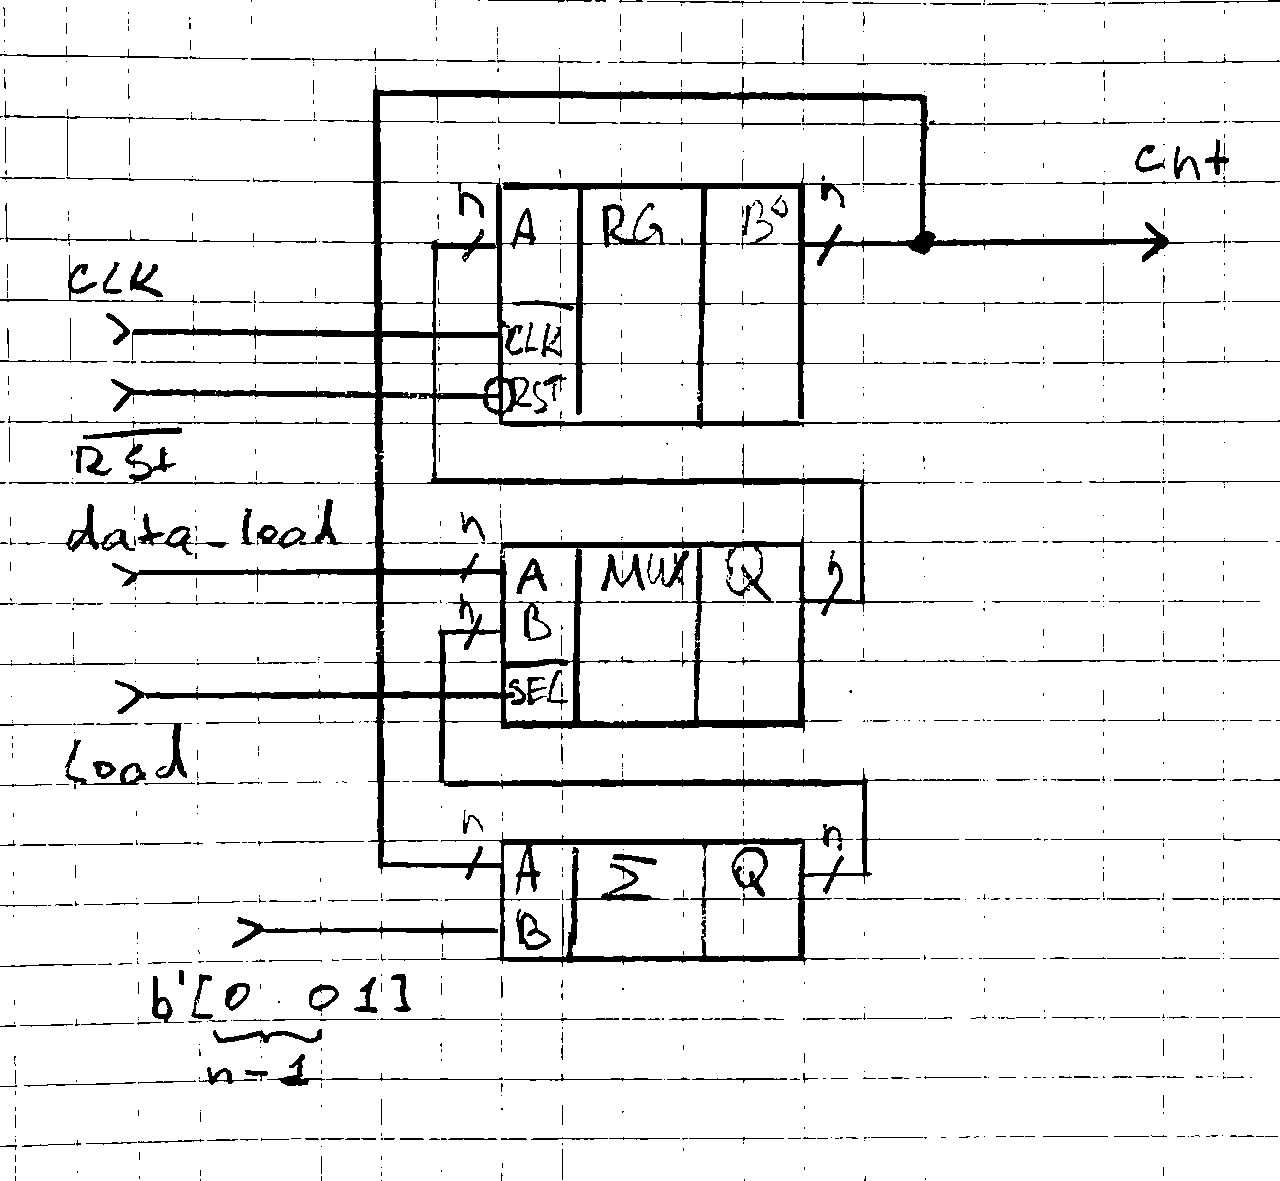
\includegraphics[width=0.5\textwidth]{lab_31}
    \caption{ЭПС счётчика с асинхронным сбросом и предустановкой}
  \end{figure}

  \begin{figure}[H]
    \centering
    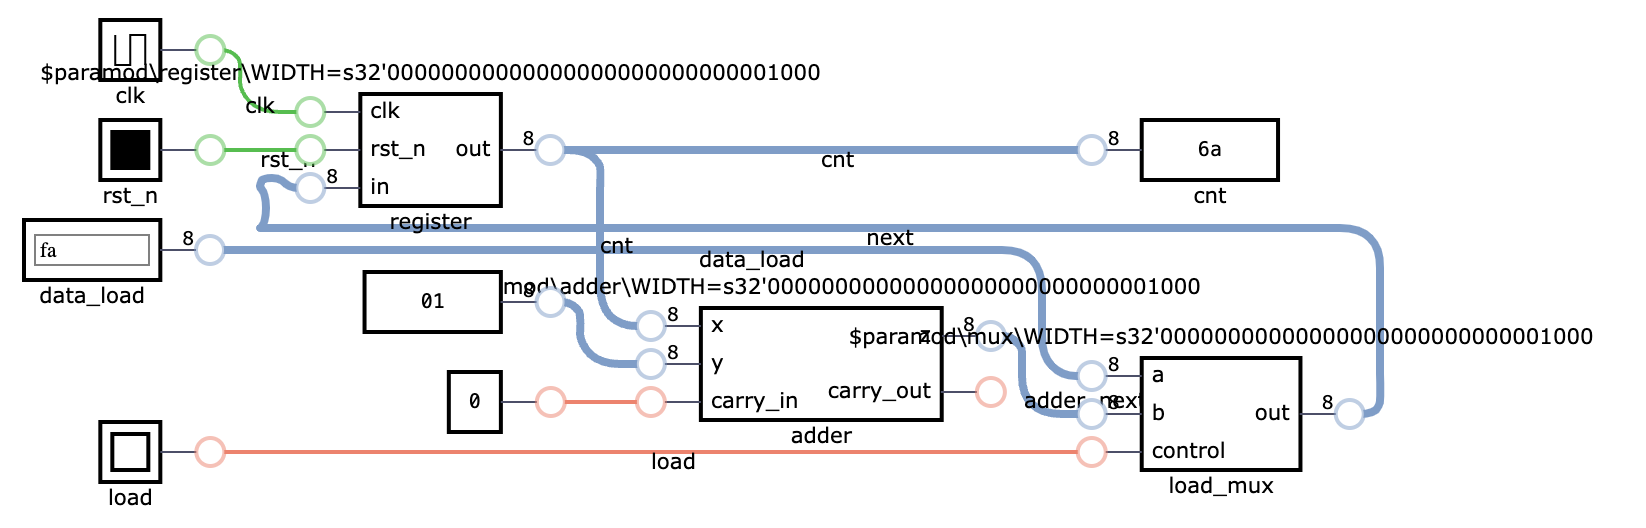
\includegraphics[width=0.8\textwidth]{lab_32}
    \caption{RTL счётчика с асинхронным сбросом и предустановкой}
  \end{figure}

  \begin{listing}[H]
    \inputminted{verilog}{../chapter_6/cnt_load/counter.v}
    \caption{Verilog описание счётчика с асинхронным сбросом и предустановкой на основе более простых элементов}
  \end{listing}

  %Аналогичное устройство может быть описано и без использования сторонних модулей:

  \begin{listing}[H]
    \begin{minted}{verilog}
      module counter #(
           parameter WIDTH=16
      ) (
        input clk,
        input rst_n,
        input load,
        input [WIDTH-1:0] data_load,
        output reg [WIDTH-1:0] cnt
      );
        always@(posedge clk or negedge rst_n)
          begin:cnt_with_load
              if(!rst_n)
                cnt <= {WIDTH{1'b0}};
              else if(load)
                cnt <= data_load;
              else
                cnt <= cnt + 1'b1;
          end
      endmodule 
    \end{minted}
    \caption{Ещё один пример реализации счётчика с асинхронным сбросом и предустановкой}
  \end{listing}

  %Тестирование модуля производилось при помощи Verilator и C++ тестбенча:

  \begin{listing}[H]
    \begin{minted}{c++}
      // ====================  Testbench   ====================

      counter->rst_n = 1;
      counter->data_load = counter->load = 0;
  
      std::cout << static_cast<int>(counter->cnt) << std::endl;
      for (int i {0}; i < 4; i++) {
          nextPeriod();
          std::cout << "+1 = " << static_cast<int>(counter->cnt) << std::endl;
      }
  
      nextStep();
      counter->rst_n = 0;
      for (int i {0}; i < CLOCK_PERIOD - 1; i++) {
          nextStep();
      }
      std::cout << "After reset = " << static_cast<int>(counter->cnt) << std::endl;
  
      counter->rst_n = 1;
      for (int i = 0; i < 4; i++) {
          nextPeriod();
      }
  
      std::cout << "Load 250" << std::endl;
      counter->data_load = 250;
      counter->load = 1;
  
      nextPeriod();
      std::cout << "Cnt = " << static_cast<int>(counter->cnt) << std::endl;
      counter->load = 0;
  
      std::cout << "Owerflow test" << std::endl;
      for (int i = {0}; i < 7; i++) {
          nextPeriod();
          std::cout << "+1 = " << static_cast<int>(counter->cnt) << std::endl;
      }
    \end{minted}
    \caption{Основная логика теста для счётчика с асинхронным сбросом и предустановкой}
  \end{listing}

  \begin{figure}[H]
    \begin{subfigure}[b]{0.75\textwidth}
      \centering
      \raisebox{1cm}{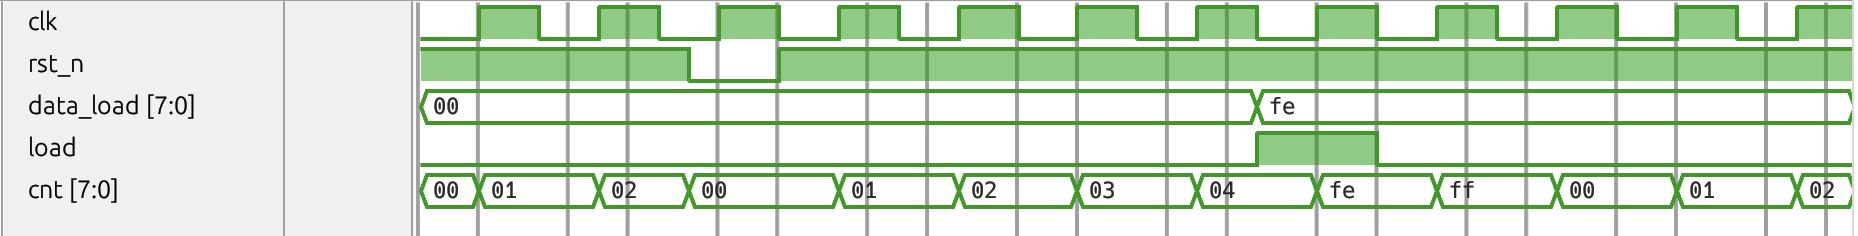
\includegraphics[width=\textwidth,height=2cm]{lab_33.png}}
    \end{subfigure}
    \hfill
    \begin{subfigure}[b]{0.2\textwidth}
      \begin{minted}{text}
        0
        +1 = 1
        +1 = 2
        After reset = 0
        Load 254
        Cnt = 254
        Owerflow test
        +1 = 255
        +1 = 0
        +1 = 1
      \end{minted}
    \end{subfigure}
    \caption{Результат работы тестбенча}
  \end{figure}

  \subsubsection{Счётчик с управляемым направлением счёта}

  Счётчики данного типа также содержат сцециальный $up_down$ вход,
  определяющий в каком направлении вести счёт - на убывание или на увеличение.

  Для построения такого счётчика необходим элемент, выполняющий вычитание
  двух чисел. Далее на схемах он будет отмечен как $SUB$, построить его можно
  на основе двух сумматоров:

  \begin{figure}[H]
    \centering
    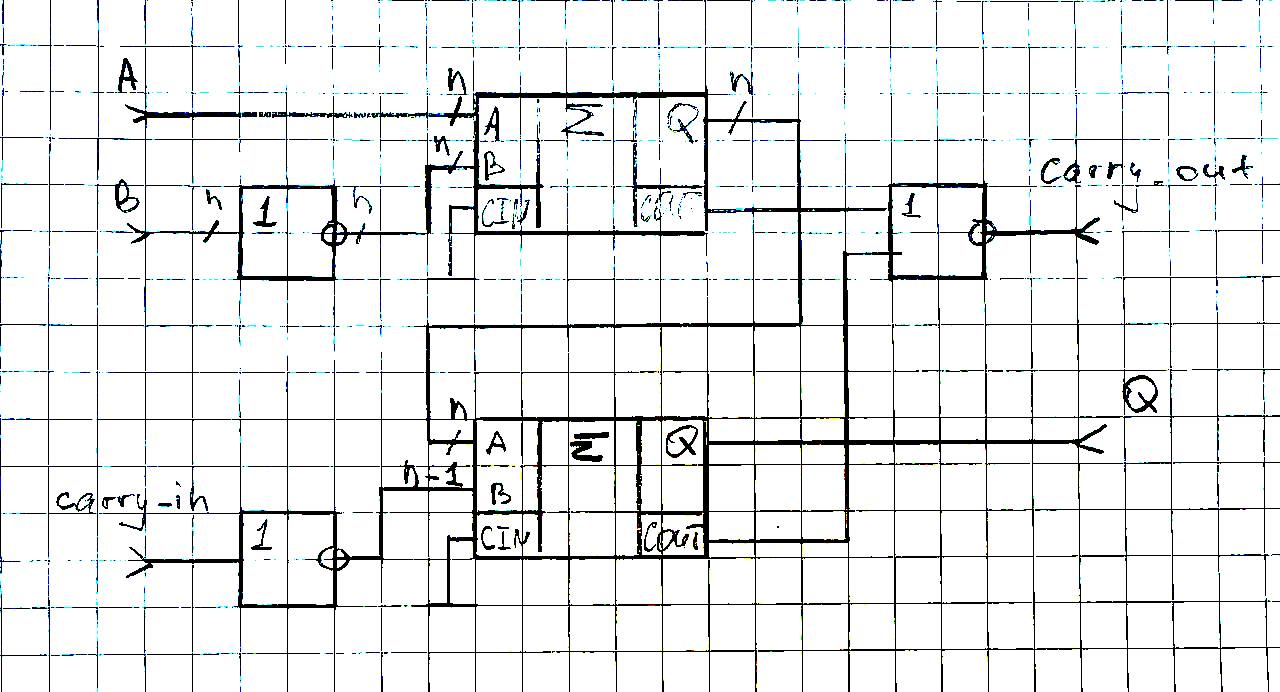
\includegraphics[width=0.7\textwidth]{lab_34.jpg}
    \caption{ЭПС для $SUB$}
  \end{figure}

  \begin{figure}[H]
   \begin{minted}{verilog}
    module substractor #(
        parameter WIDTH = 8
    ) (
        input [WIDTH - 1 : 0] x,
        input [WIDTH - 1 : 0] y,
        input carry_in,
        output [WIDTH - 1 : 0] z,
        output carry_out
    );
      wire [WIDTH - 1 : 0] carry;
      wire carry_adder, carry_coder;

      adder #(.WIDTH (WIDTH)) adder (
        .x (x),
        .y (~ y),
        .carry_in (0),
        .z (carry),
        .carry_out (carry_adder)
      );
      adder #(.WIDTH (WIDTH)) coder (
        .x (carry),
        .y (~ carry_in),
        .carry_in (0),
        .z (z),
        .carry_out (carry_coder)
      );
      assign carry_out = (~ carry_coder) & (~ carry_adder);
    endmodule
   \end{minted} 
   \caption{Реализация $SUB$}
  \end{figure}

  Теперь можно собрать счётчик с управляемым направлением счёта при
  помощи более простых элементов:

  \begin{figure}[H]
    \begin{subfigure}[b]{0.37\textwidth}
    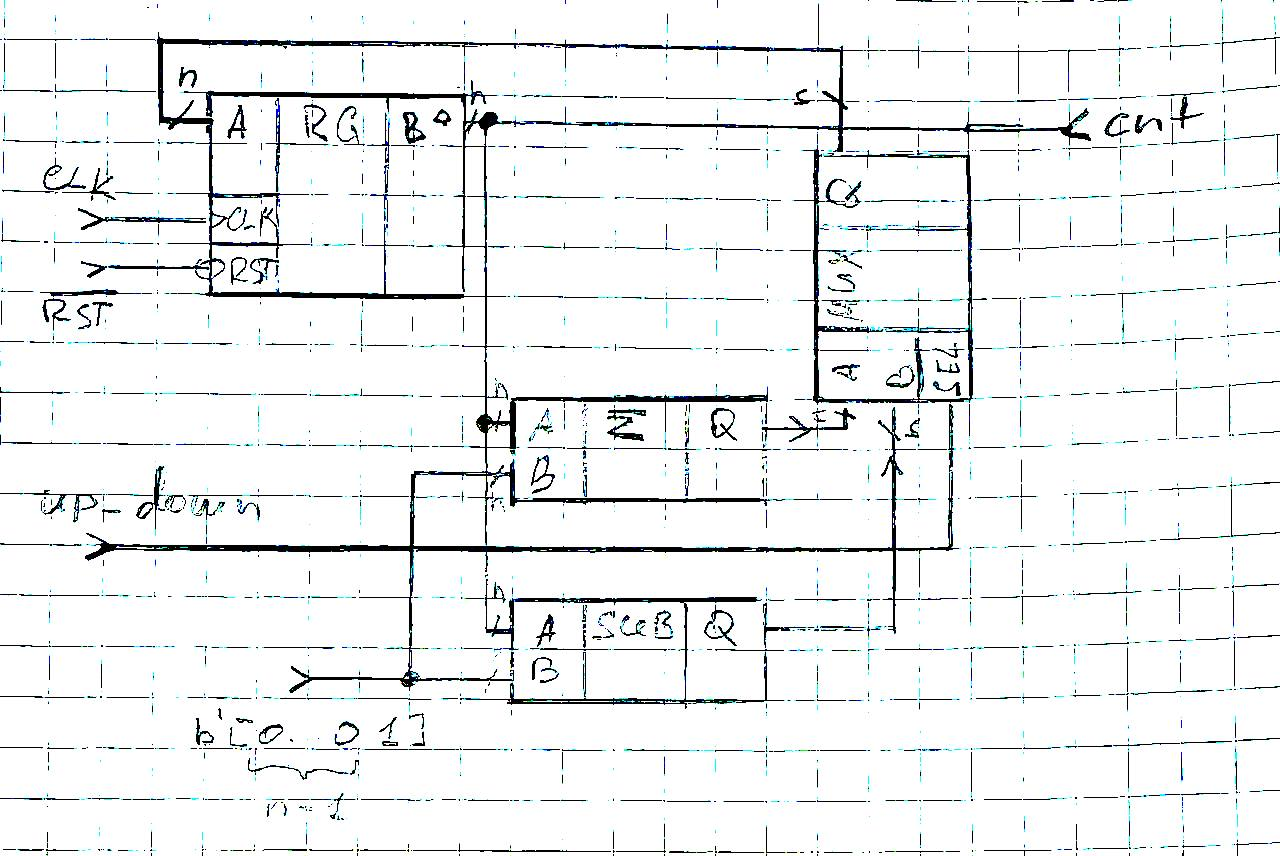
\includegraphics[width=0.9\textwidth]{lab_35.jpg}
    \end{subfigure}
    \hfill
    \begin{subfigure}[b]{0.6\textwidth}
    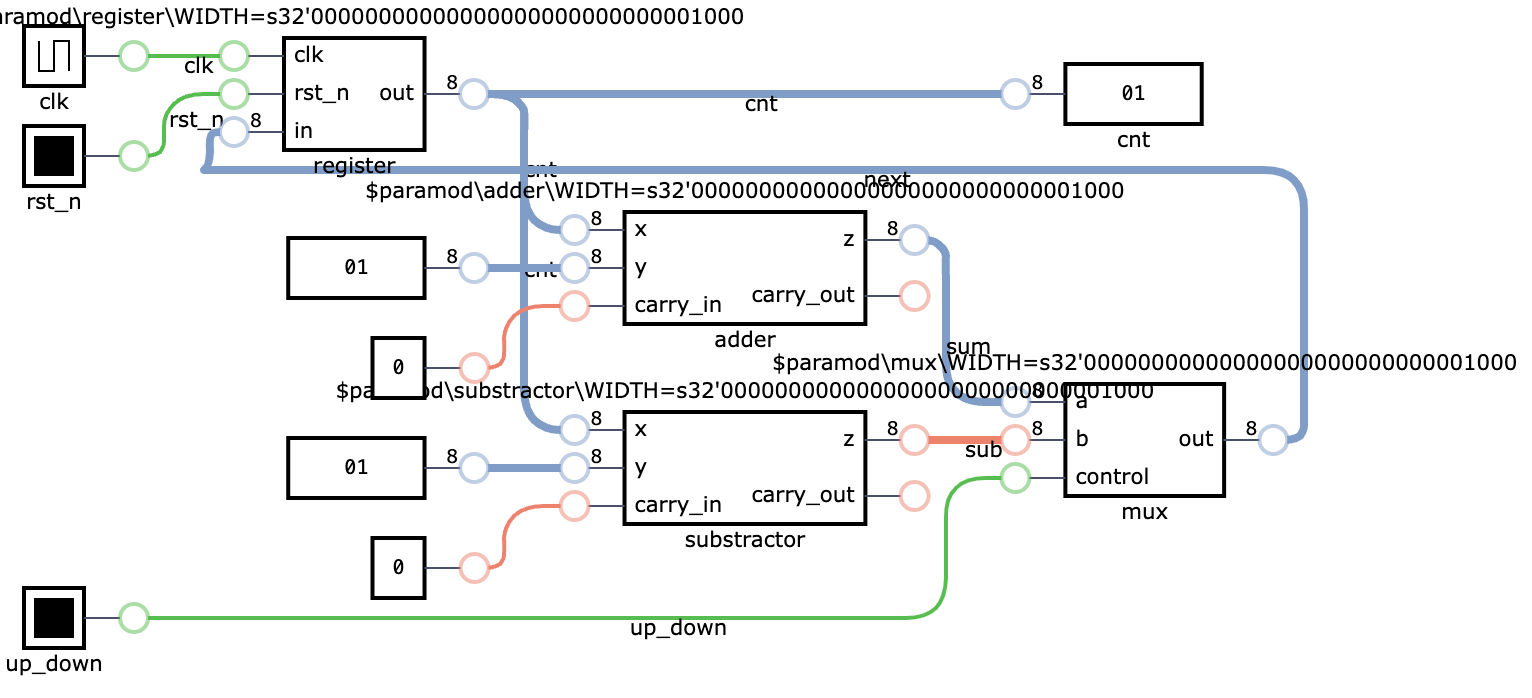
\includegraphics[width=0.8\textwidth]{lab_36.png}
    \end{subfigure}
    \caption{ЭПС и RTL счётчика с управляемым направлением счёта}
  \end{figure}

  \begin{listing}[H]
    \inputminted{verilog}{../chapter_6/cnt_ud/counter.v}
    \caption{Verilog описание счётчика с управляемым направлением счёта}
  \end{listing}

  \begin{listing}[H]
    \begin{minted}{verilog}
      module cnt_updown #( 
          parameter WIDTH=16
      ) (
          input clk,
          input rst_n,
          input up_down, 
          output reg [WIDTH-1:0] cnt
      );
        always@(posedge clk or negedge rst_n)
          begin
              if(!rst_n)
                cnt <= {WIDTH{1'b0}};
              else if(up_down)
                cnt <= cnt + 1'b1;
              else
                cnt <= cnt - 1'b1;
          end
      endmodule // cnt_updown
    \end{minted}
    \caption{Альтернативное Verilog описание без использования дополнительных модулей}
  \end{listing}

  \begin{listing}[H]
    \begin{minted}{c++}
      // ====================  Testbench   ====================

      counter->rst_n = counter->up_down = 1;
  
      std::cout << static_cast<int>(counter->cnt) << std::endl;
      for (int i {0}; i < 2; i++) {
          nextPeriod();
          std::cout << "+1 = " << static_cast<int>(counter->cnt) << std::endl;
      }
  
      counter->up_down = 0;
      for (int i {0}; i < 4; i++) {
          nextPeriod();
          std::cout << "-1 = " << static_cast<int>(counter->cnt) << std::endl;
      }
  
      nextStep();
      counter->rst_n = 0;
      for (int i {0}; i < CLOCK_PERIOD - 1; i++) {
          nextStep();
      }
      std::cout << "After reset = " << static_cast<int>(counter->cnt) << std::endl;
    \end{minted}
    \caption{Основной код тестбенча для счётчика с управляемым направлением сброса} 
  \end{listing}

  \begin{figure}[H]
    \begin{subfigure}[b]{0.75\textwidth}
      \centering
      \raisebox{0.75cm}{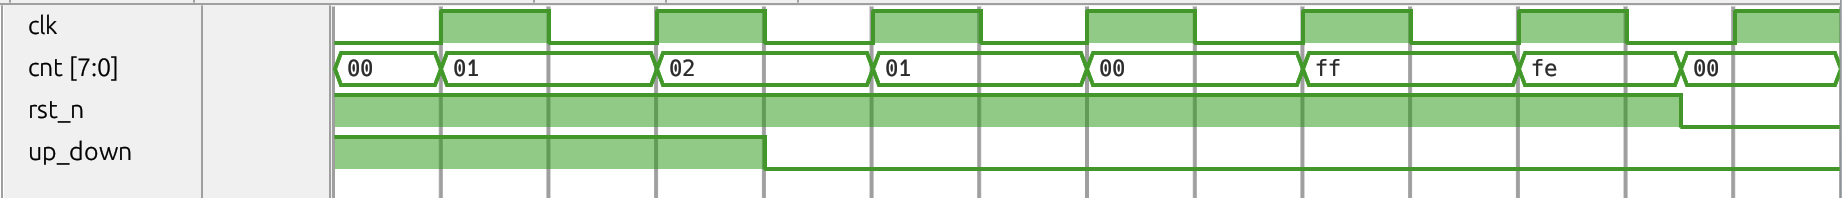
\includegraphics[width=\textwidth,height=2cm]{lab_37.png}}
    \end{subfigure}
    \hfill
    \begin{subfigure}[b]{0.2\textwidth}
      \begin{minted}{text}
        0
        +1 = 1
        +1 = 2
        -1 = 1
        -1 = 0
        -1 = 255
        -1 = 254
        After reset = 0
      \end{minted}
    \end{subfigure}
    \caption{Результат работы тестбенча}
  \end{figure}

  \subsubsection{Делитель частоты}

  Делители частоты предназначены для кратного уменьшения частоты входного сигнала
  (тут частота - количество циклических колебаний в секунду). Они строятся на основе
  счётчиков (и компараторов) - вместо того, чтобы выполнять переключение выходного
  сигнала каждый тактирующий цикл, изменение уровня происходит каждые N событий
  из списка чувствительности.

  \begin{figure}[H]
    \centering
    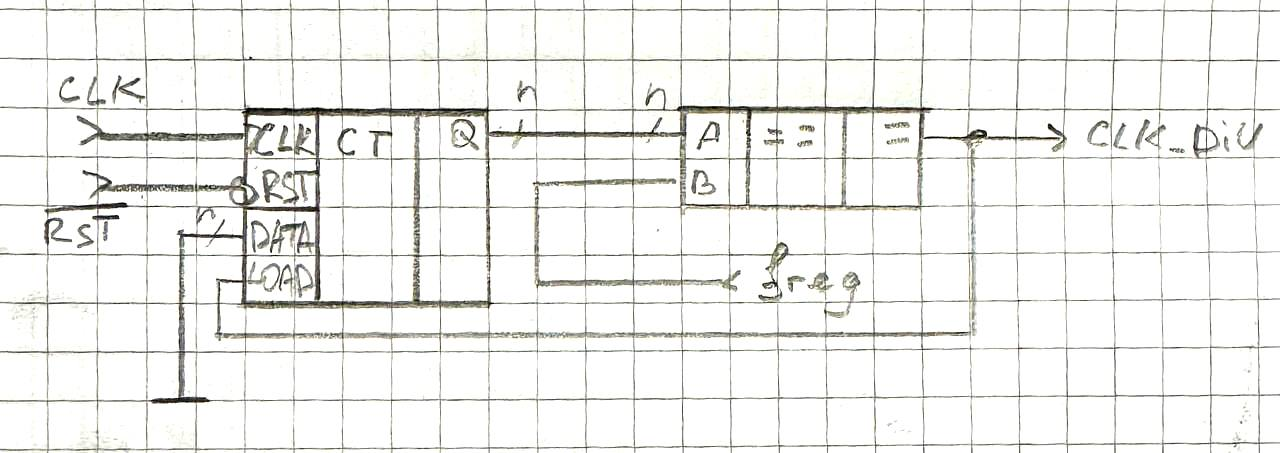
\includegraphics[width=0.7\textwidth]{lab_38.jpg} 
    \caption{ЭПС делителя частоты (на значение $freq$)}   
  \end{figure}

  \begin{figure}[H]
    \centering
    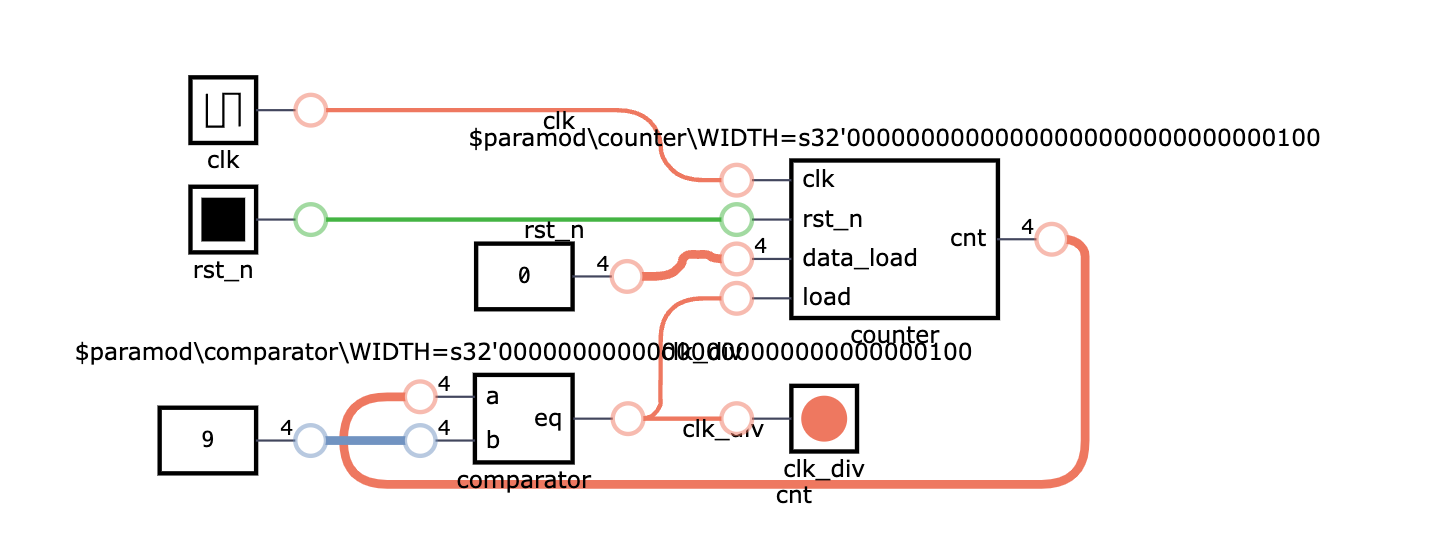
\includegraphics[width=0.8\textwidth]{lab_39.png}
    \caption{RTL делителя частоты на 10}
  \end{figure}

  \begin{listing}[H]
    \inputminted{verilog}{../chapter_6/freq_div/divider.v}
    \caption{Verilog-описание делителя частоты на $N$}
  \end{listing}

  \begin{listing}[H]
    \begin{minted}{verilog}
      module cnt_div #(
          parameter DIV_CNT=10,
          parameter WIDTH = $clog2(DIV_CNT)
      ) (
          input  clk_in,
          input  rst_n,
          output clk_out
      );
        reg [WIDTH-1:0] cnt;

        always@(posedge clk_in or negedge rst_n)
          begin
              if(!rst_n)
                cnt <= {WIDTH{1'b0}};
              else if(cnt == DIV_CNT-1)
                cnt <= {WIDTH{1'b0}};
              else
                cnt <= cnt + 1'b1;
          end
        
        assign clk_out = (cnt == 0) ? 1'b1 : 1'b0;        
      endmodule // cnt_div
    \end{minted}
    \caption{Verilog описание делителя частоты на $N$ без использования дополнительных модулей}
  \end{listing}

  \begin{listing}[H]
    \begin{minted}{cpp}
      std::cout << "N = " << NDIV << std::endl;
      divider->rst_n = 1;

      for (int i {0}; i < 10; i++) {
          for (int j {0}; j < NDIV; j++) {
              nextPeriod();
              if (divider->clk_div) {
                  std::cout << "#";
              } else {
                  std::cout << "_";
              }
          }
          std::cout << std::endl;
      }
    \end{minted}
    \caption{Основной тестбенч для делителя частоты}
  \end{listing}

  Тут $NDIV$ - это значение, в которое будет уменьшена частота тактирующего сигнала. В
  модуле на verilog оно задано как $parameter$, то есть в тестбенче его можно менять только
  с полной пересборкой. Специальный $Makefile$ считывает значение $N$, и подставляет его при
  сборке в качестве \mintinline{cpp}|#define NDIV|.

  Коэффициент заполнения выходного сигнала можно посчитать по формуле $1 / N$ (некий аналог скважности),
  то есть при $N = 2$, мы получим заполнение в $50\%$, при $N = 4$ - $25\%$, при $N = 5$ - $20\%$ и т.д.

  \begin{figure}[H]
    \begin{subfigure}[b]{0.75\textwidth}
      \centering
      \raisebox{0.25cm}{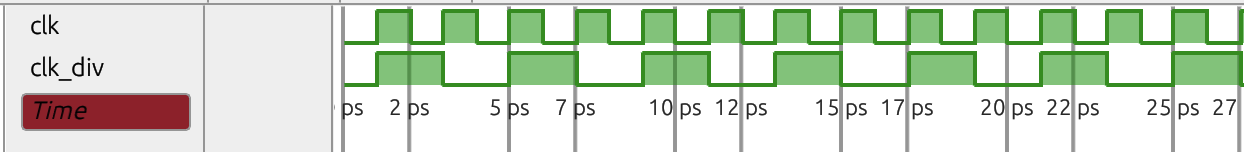
\includegraphics[width=\textwidth,height=2cm]{lab_310.png}}
    \end{subfigure}
    \hfill
    \begin{subfigure}[b]{0.2\textwidth}
      \begin{minted}{text}
        N = 2
        #_
        #_
        #_
        #_
      \end{minted}
    \end{subfigure}
    \caption{Результат работы тестбенча (деление частоты на 2)}
  \end{figure}

  \begin{figure}[H]
    \begin{subfigure}[b]{0.75\textwidth}
      \centering
      \raisebox{0.25cm}{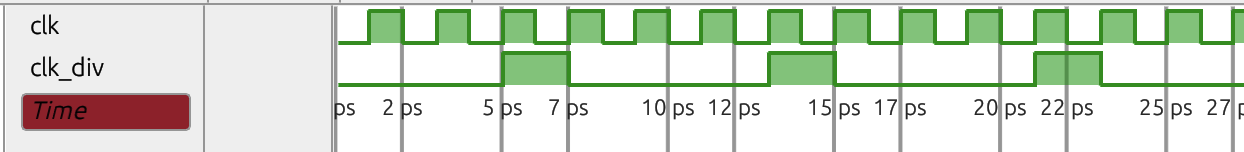
\includegraphics[width=\textwidth,height=2cm]{lab_311.png}}
    \end{subfigure}
    \hfill
    \begin{subfigure}[b]{0.2\textwidth}
      \begin{minted}{text}
        N = 4
        __#_
        __#_
        __#_
        __#_
      \end{minted}
    \end{subfigure}
    \caption{Результат работы тестбенча (деление частоты в 4 раза)}
  \end{figure}

  \begin{figure}[H]
    \begin{subfigure}[b]{0.75\textwidth}
      \centering
      \raisebox{0.25cm}{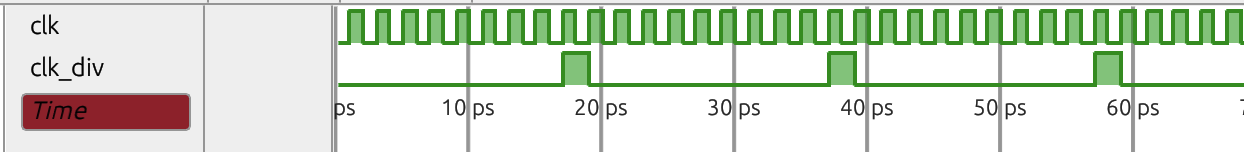
\includegraphics[width=\textwidth,height=2cm]{lab_312.png}}
    \end{subfigure}
    \hfill
    \begin{subfigure}[b]{0.2\textwidth}
      \begin{minted}{text}
        N = 10
        ________#_
        ________#_
        ________#_
        ________#_
      \end{minted}
    \end{subfigure}
    \caption{Результат работы тестбенча (деление частоты в 10 раз)}
  \end{figure}

  \subsubsection{Широтно-Импульсная Модуляция}

  ШИМ позволяет регулировать мощность изменяя длительность импульса и длительность паузы (задержка между импульсами).
  Чем больше длительность импульса относительно длительности паузы, тем выше мощность (тут скважность - отношение
  длительности импульса к длительности паузы).

  На самом деле делитель частоты - самый простой ШИМ, но он не умеет изменять длительность импульса, только скважность.

  \begin{figure}[H]
    \begin{subfigure}[b]{0.45\textwidth}
    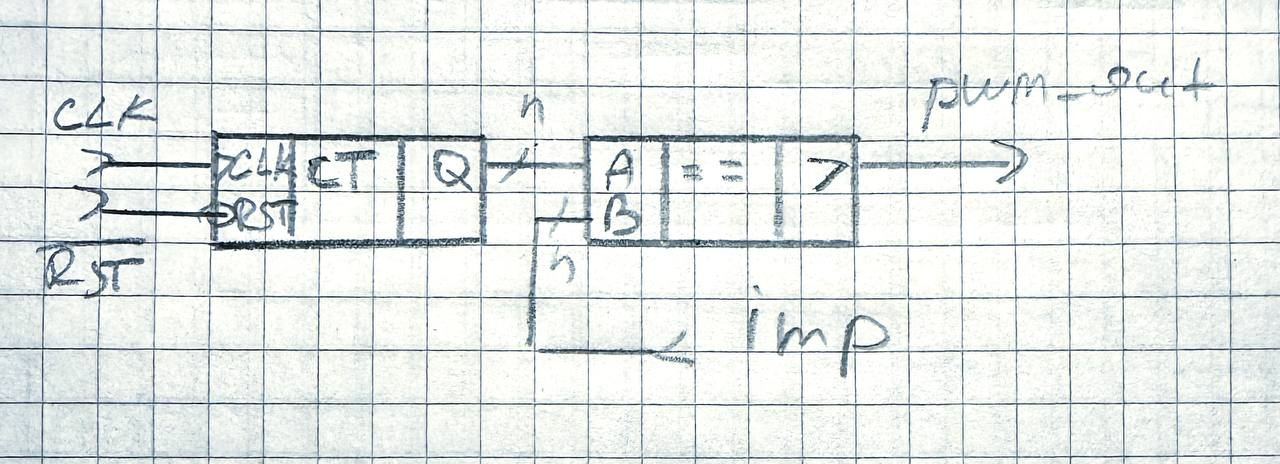
\includegraphics[width=0.9\textwidth]{lab_313}
    \end{subfigure}
    \hfill
    \begin{subfigure}[b]{0.45\textwidth}
    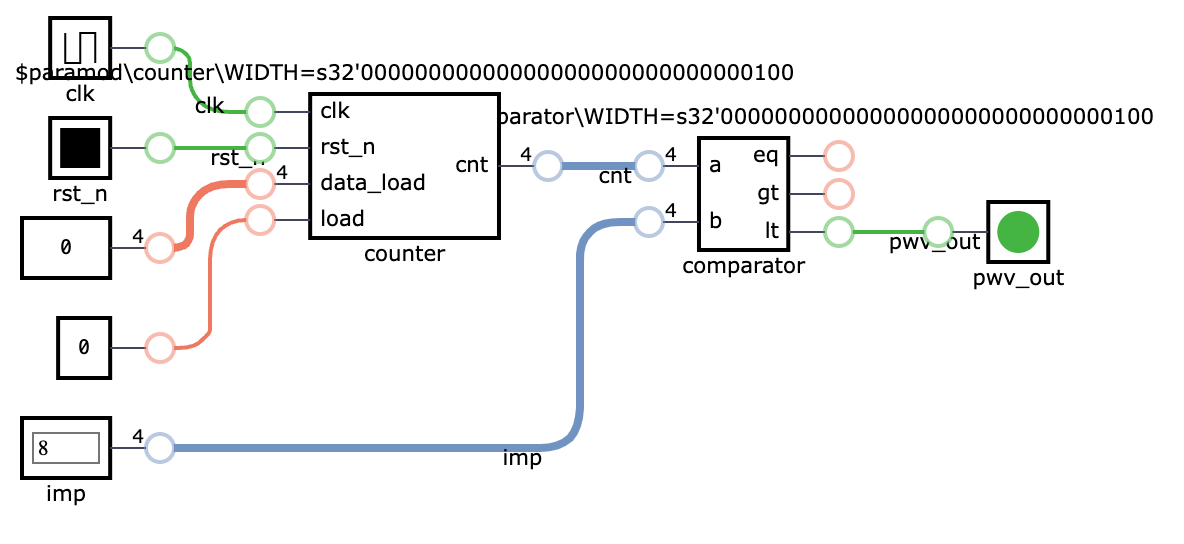
\includegraphics[width=0.9\textwidth]{lab_314}
    \end{subfigure}
    \caption{ЭПС и RTL модуля ШИМ}
  \end{figure}

  \begin{listing}[H]
    \inputminted{verilog}{../chapter_6/pwm/pwm.v}
    \caption{Реализация ШИМ-модуля}
  \end{listing}

  \begin{listing}[H]
    \begin{minted}{verilog}
      module pwm #(
           parameter PWM_WIDTH=16
      ) (
           input clk,
           input rst_n,
           input [PWM_WIDTH-1:0] imp_width,
           output pwm_out
       );
         reg [PWM_WIDTH-1:0] cnt;
         
         always@(posedge clk or negedge rst_n)
           begin
              if(!rst_n)
                cnt <= {PWM_WIDTH{1'b0}};
              else
                cnt <= cnt + 1'b1;
           end
         assign pwm_out = (imp_width > cnt) ? 1'b1 : 1'b0;
      endmodule // pwm
    \end{minted}
    \caption{Реализация ШИМ без использования дополнительный модулей}
  \end{listing}

  \begin{listing}[H]
    \begin{minted}{cpp}
      // ====================  Testbench   ====================

      std::cout << "PWD_WIDTH = " << PWD_WIDTH << std::endl;
      pwm->rst_n = 1;

      for (int i {0}; i <= (1 << PWD_WIDTH); i++) {
          std::cout << "(" << i << " / " << (1 << PWD_WIDTH) << ") ";
          pwm->imp = i;
          for (int j {0}; j < 3 * (1 << PWD_WIDTH); j++) {
              nextPeriod();
              std::cout << (pwm->pwv_out ? '#' : '_');
          }
          std::cout << std::endl;
      }
    \end{minted}
    \caption{Код тестбенча}
  \end{listing}
  
  \begin{figure}[H]
    \begin{subfigure}[b]{0.75\textwidth}
      \centering
      \raisebox{0.35cm}{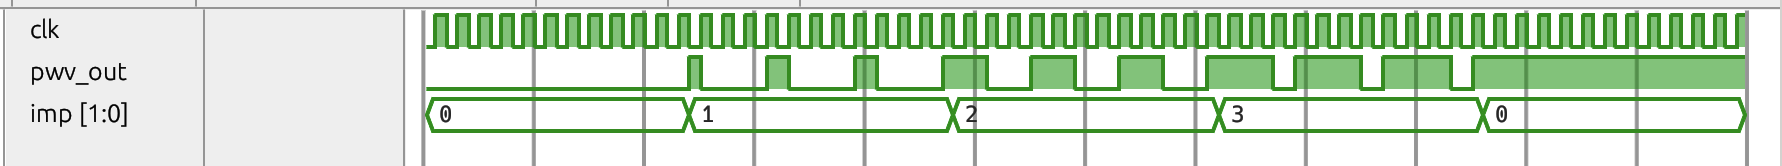
\includegraphics[width=\textwidth,height=2cm]{lab_315}}
    \end{subfigure}
    \hfill
    \begin{subfigure}[b]{0.2\textwidth}
      \begin{minted}{text}
        PWD_WIDTH = 2
        (0 / 4) ____________
        (1 / 4) ___#___#___#
        (2 / 4) #__##__##__#
        (3 / 4) ##_###_###_#
        (4 / 4) ############
      \end{minted}
    \end{subfigure}
    \caption{Результат работы ШИМ}
  \end{figure}

  \subsubsection{Код Грея}

  Код Грея - двоичный код, в котором расстояние Хэмминга между двумя соседними
  числами всегда равно $1$. Чтобы перевести число в двоичной системе счисления
  в код Грея, необходимо:
  \begin{equation}
    n_{gray} = n_2 \oplus (n_2 >> 1)
  \end{equation}

  Счётчик Грея - счётчик, выход которого описывает число не бинарным кодом, а кодом Грея.

  \begin{listing}[H]
    \inputminted{verilog}{../chapter_6/bin2gray.v}
    \caption{Verilog описание перевода бинарного кода в код Грея}
  \end{listing}

  \begin{figure}[H]
    \begin{subfigure}[b]{0.25\textwidth}
    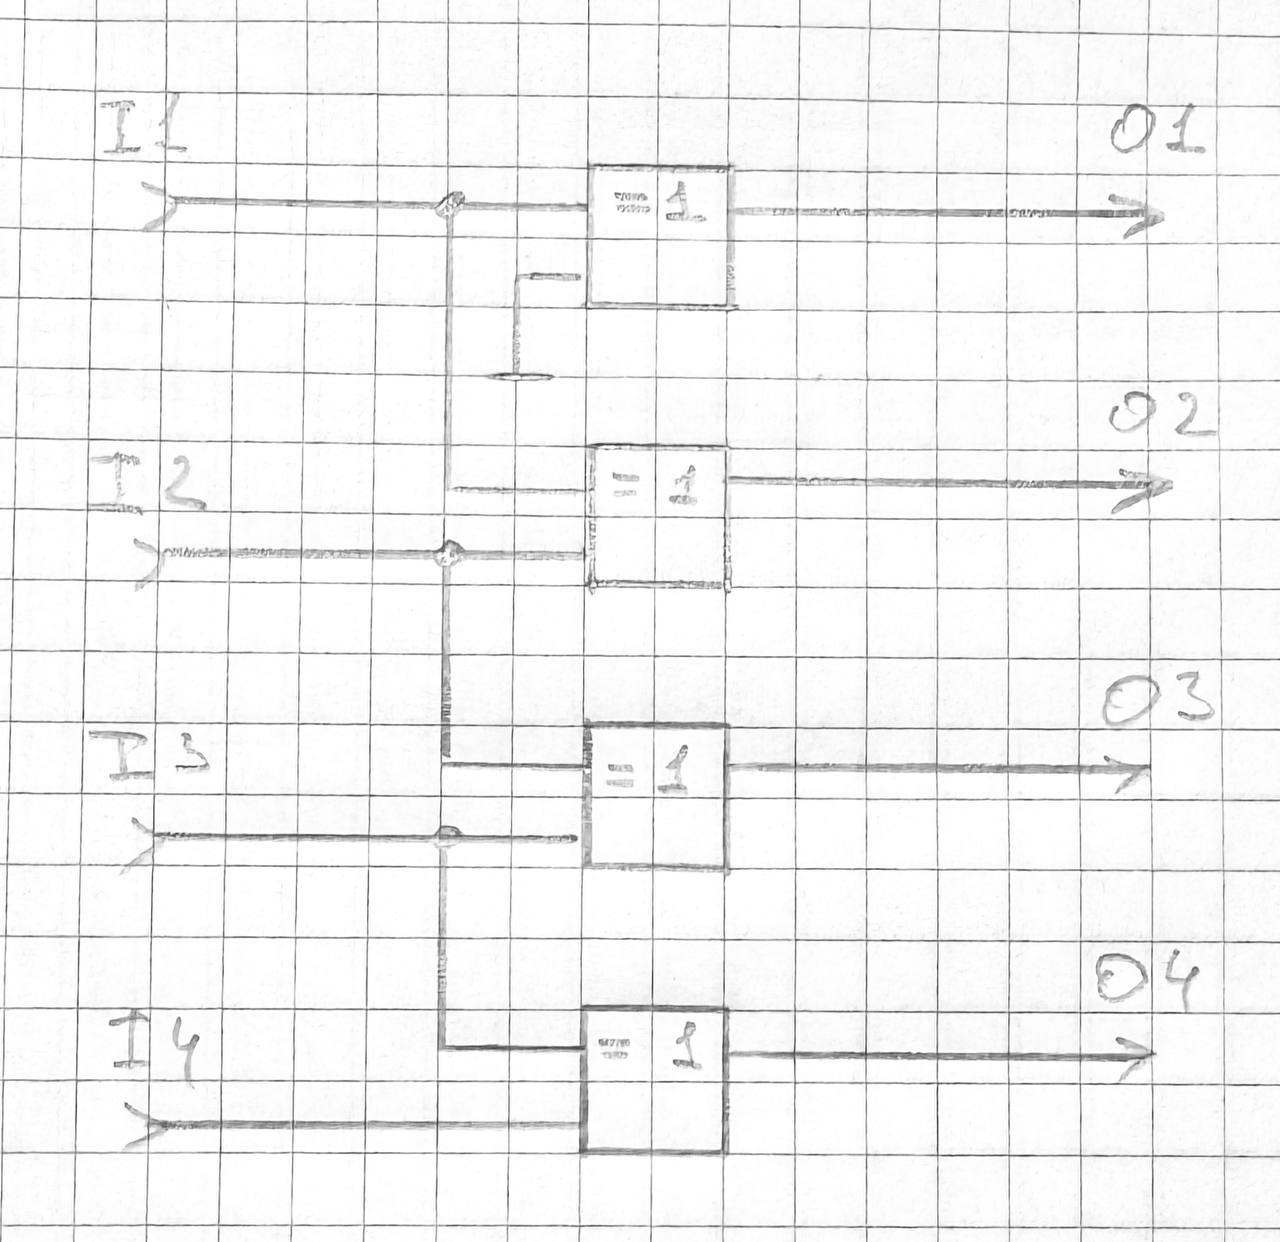
\includegraphics[width=0.9\textwidth]{lab_316}
    \end{subfigure}
    \hfill
    \begin{subfigure}[b]{0.7\textwidth}
    \raisebox{0.75cm}{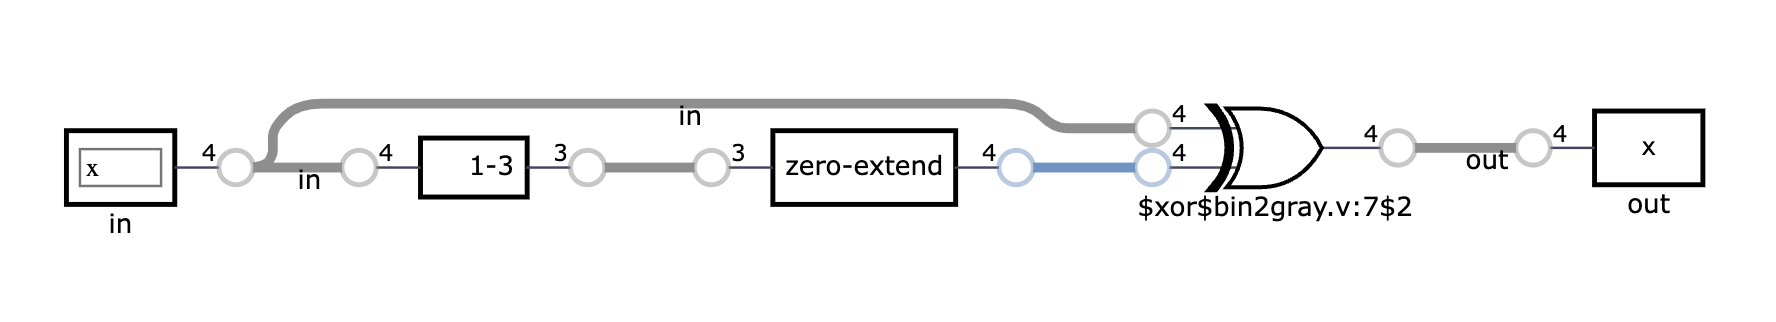
\includegraphics[width=0.9\textwidth]{lab_317}}
    \end{subfigure}
    \caption{ЭПС и RTL конвертора бинарного кода в код Грея}
  \end{figure}

  \begin{figure}[H]
    \centering
    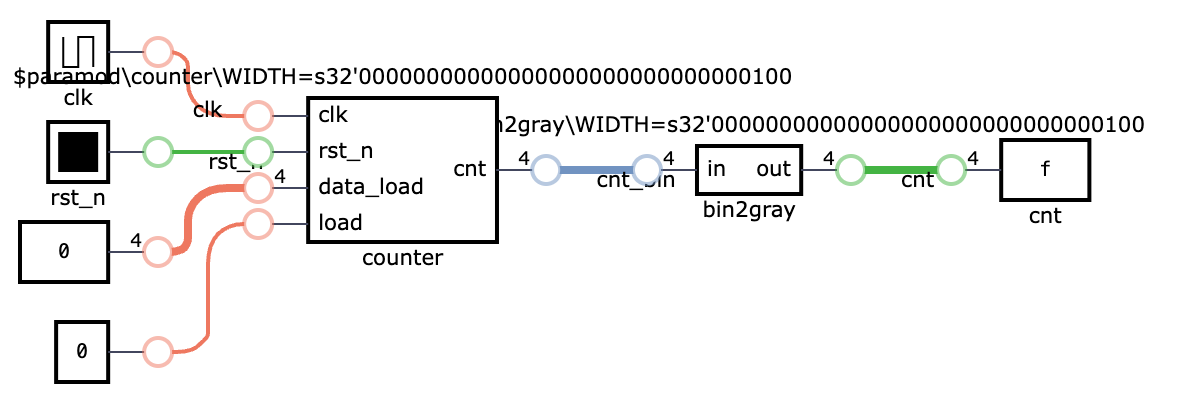
\includegraphics[width=0.6\textwidth]{lab_318}
    \caption{RTL счётчика Грея}
  \end{figure}

  \begin{listing}[H]
    \inputminted{verilog}{../chapter_6/gray_cnt/gray_counter.v}
    \caption{Verilog описание счётчика Грея}
  \end{listing}

  \begin{listing}[H]
    \begin{minted}{cpp}
// ====================  Testbench   ====================

std::cout << "NWIDTH = " << NWIDTH << std::endl;
gray->rst_n = 1;

for (int i {0}; i < (1 << NWIDTH); i++) {
    std::cout << "(" << i << " / " << (1 << NWIDTH) << ") ";
    std::cout << std::setw(4) << std::setfill('0') << toBin(gray->cnt) << std::endl;
    nextPeriod();
}
    \end{minted}
    \caption{Код тестбенча}
  \end{listing}

  \begin{figure}[H]
    \centering
    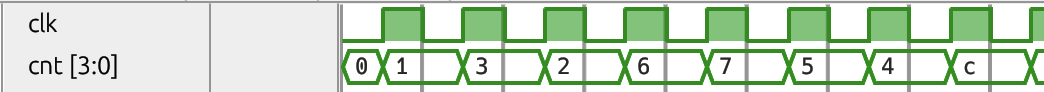
\includegraphics[width=0.8\textwidth]{lab_319.png}
    \caption{Результат работы тестбенча}
  \end{figure}

  \begin{listing}[H]
    \begin{minted}{text}
NWIDTH = 4
(0 / 16) 0000
(1 / 16) 0001
(2 / 16) 0011
(3 / 16) 0010
(4 / 16) 0110
(5 / 16) 0111
    \end{minted}
    \caption{Результат работы тестбенча}
  \end{listing}

  \subsubsection{Сдвиговый регистр}

  Сдвиговый регистр позволяет выполнять операцию сдвига на 1 бит. Состоит из нескольких
  последовательно соединённых D-триггеров с единым тактирующим сигналом.

  \begin{figure}[H]
    \centering
    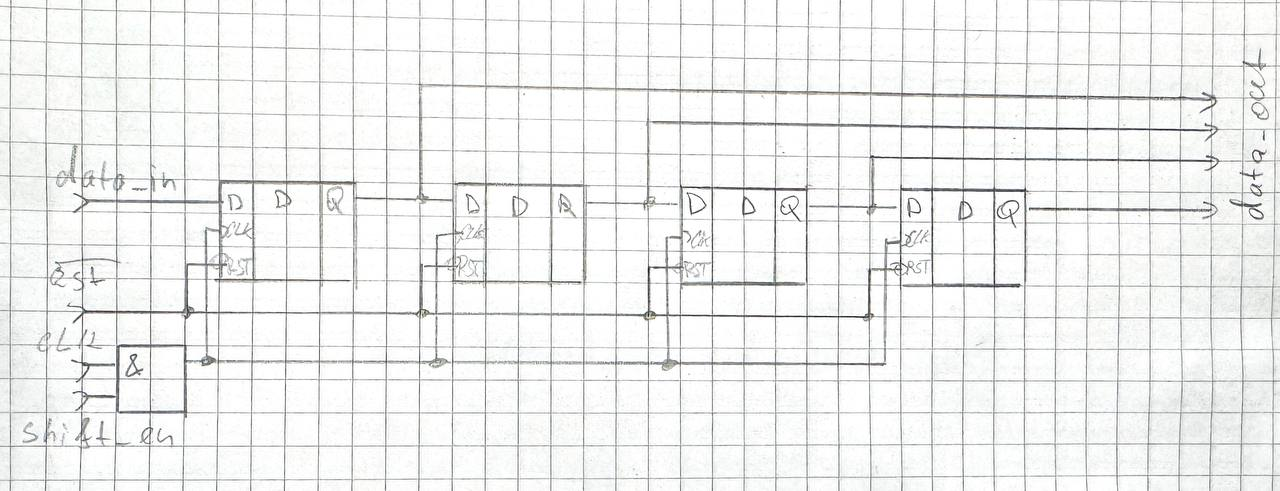
\includegraphics[width=0.9\textwidth]{lab_320.jpg}
    \caption{ЭПС сдвигового регистра на 4 разряда}
  \end{figure}

  \begin{figure}[H]
    \centering
    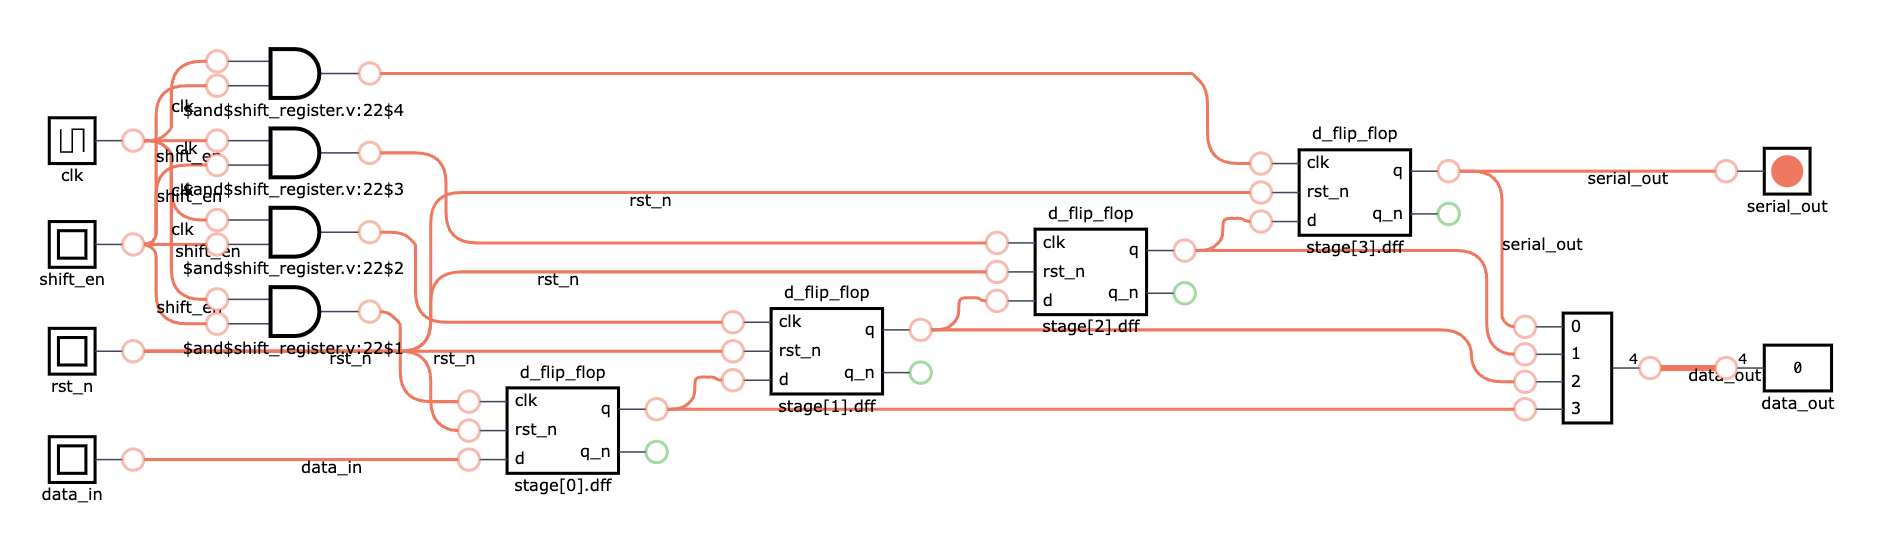
\includegraphics[width=0.9\textwidth]{lab_321}
    \caption{RTL сдвигового регистра на 4 разряда}
  \end{figure}

  \begin{listing}[H]
    \inputminted{verilog}{../chapter_6/shift_reg/shift_register.v}
    \caption{Verilog-описание сдвигового регистра}
  \end{listing}

  \begin{listing}[H]
    \begin{minted}{verilog}
// ====================  Testbench   ====================

std::cout << "WIDTH = " << WIDTH << std::endl;
sr->rst_n = 1; sr->shift_en = 1;

for (int i {0}; i <= WIDTH * 3; i++) {
    sr->data_in = (i % 3 == 2 ? 0 : 1);
    std::cout << "(" << std::setw(2) << std::setfill(' ') << i << " / " << (1 << WIDTH) << ") "
        << "+" << static_cast<int>(sr->data_in) << " " << (sr->shift_en ? " on" : "off") << " ";
    nextPeriod();
    std::cout << std::setw(WIDTH) << std::setfill('0') << toBin(sr->data_out) << std::endl;
    if (i == WIDTH * 2) sr->shift_en = 0;
}
    \end{minted}
    \caption{Тестбенч регистра}
  \end{listing}

  \begin{listing}[H]
    \begin{minted}{text}
WIDTH = 4
( 0 / 16) +1  on 1000
( 1 / 16) +1  on 1100
( 2 / 16) +0  on 0110
( 3 / 16) +1  on 1011
( 4 / 16) +1  on 1101
( 5 / 16) +0  on 0110
( 6 / 16) +1  on 1011
( 7 / 16) +1  on 1101
( 8 / 16) +0  on 0110
( 9 / 16) +1 off 0110
(10 / 16) +1 off 0110
(11 / 16) +0 off 0110
(12 / 16) +1 off 0110
    \end{minted}
    \caption{Результат работа тестбенча}
  \end{listing}

  \begin{figure}[H]
    \centering
    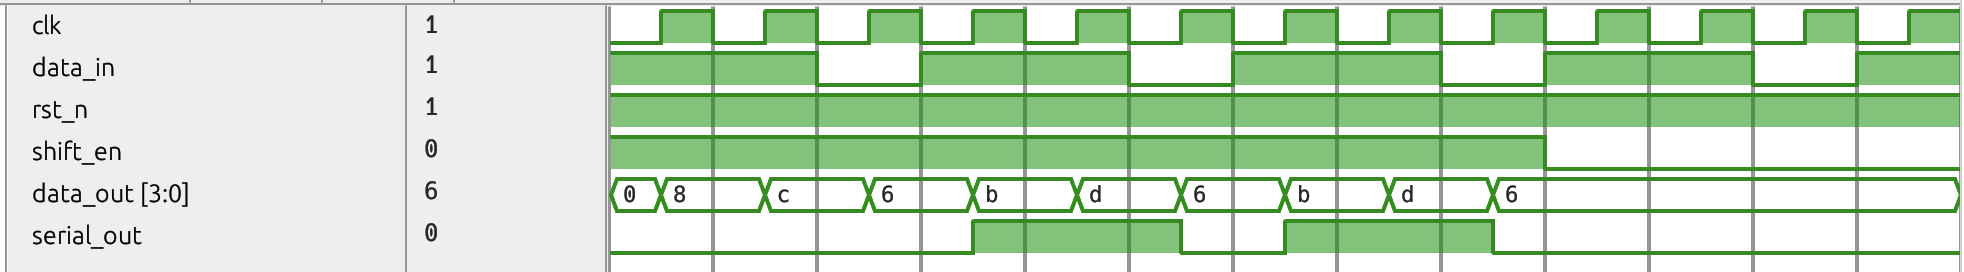
\includegraphics[width=0.9\textwidth]{lab_322.png}
    \caption{Результат работа тестбенча}
  \end{figure}

  \newpage
  \section{Дополнительные задания}

  В данном разделе реализуются модули, взаимодействующие с семисегментными
  индикаторами, расположенными на ПЛИС. Платы у меня нет, но есть C++, на котором
  написана небольшая обёртка-эмулятор над группой из нескольких последовательных
  индикаторов:

  \begin{listing}[H]
    \begin{minted}{cpp}
      std::array<std::string, 4> ledToView(int8_t led) {
          std::array<std::string, 4> view;

          view[0] = " " + std::string {(~led & 0b00000001) ? "_" : " "} + " ";
          view[1] = std::string {(~led & 0b00100000) ? "|" : " "} + 
                    std::string {(~led & 0b01000000) ? "_" : " "} +
                    std::string {(~led & 0b00000010) ? "|" : " "};
          view[2] = std::string {(~led & 0b00010000) ? "|" : " "} +
                " " + std::string {(~led & 0b00000100) ? "|" : " "};
          view[3] = " " + std::string {(~led & 0b00001000) ? "‾" : " "} + " "; 

          return view;
      }

      void printViews(const std::vector<std::array<std::string, 4>>& d) {
          for (int i {0}; i < 4; i++) {
              for (const auto& a : d) {
                  std::cout << a[i];
              }
              std::cout << std::endl;
          }
      }

      void printLedsWire(std::int64_t wire, std::size_t leds_num = LEDS) {
          std::vector<std::array<std::string, 4>> leds;

          for (int i {0}; i < leds_num; i++) {
              std::int8_t l = static_cast<std::int8_t>((wire >> (8 * (leds_num - i - 1))) & 0xff);
              leds.push_back(ledToView(l));
          }

          printViews(leds);   
      }
    \end{minted}
    \caption{Вспомогательные функции для эмуляции N-семисегментных индикаторов}
  \end{listing}

  Данный код работает с приложенным к лабораторной работе led7.v модулем
  и предназначен для использования в тестбенчах.

  \subsection{Отображение значения со счётчика на группе семисегментных индикаторов в десятичном формате (задание 1)}

  На выходе счётчика мы получаем бинарное представление его внутреннего
  значения. Если подать это представление на дешифратор для семисегментного
  индикатора (модуль led7), то мы увидим посчитанное значение, но в шестнадцетеричном формате.
  Для того, чтобы произвести отображение в привычной нам десятичной системе
  счисления, необходимо преобразовать бинарный код с выхода счётчика в
  двоично-десятичный код:

  \begin{listing}[H]
    \inputminted{verilog}{../chapter_6/bin2bcd.v}
    \caption{Конвертор двоичного кода в двоично-десятичный}
  \end{listing}

  Перевод происходит при помощи Double Dabble алгоритма.
  Теперь мы можем соединить счётчик с семисегментными индикаторами и увидеть
  его значение в десятичной системе счисления:
  
  \begin{listing}[H]
    \inputminted{verilog}{../chapter_6/extra/1/task1.v}
    \caption{Счётчик соединённый с группой из 6 семисегментных индикаторов}
  \end{listing}

  \begin{figure}[H]
    \centering
    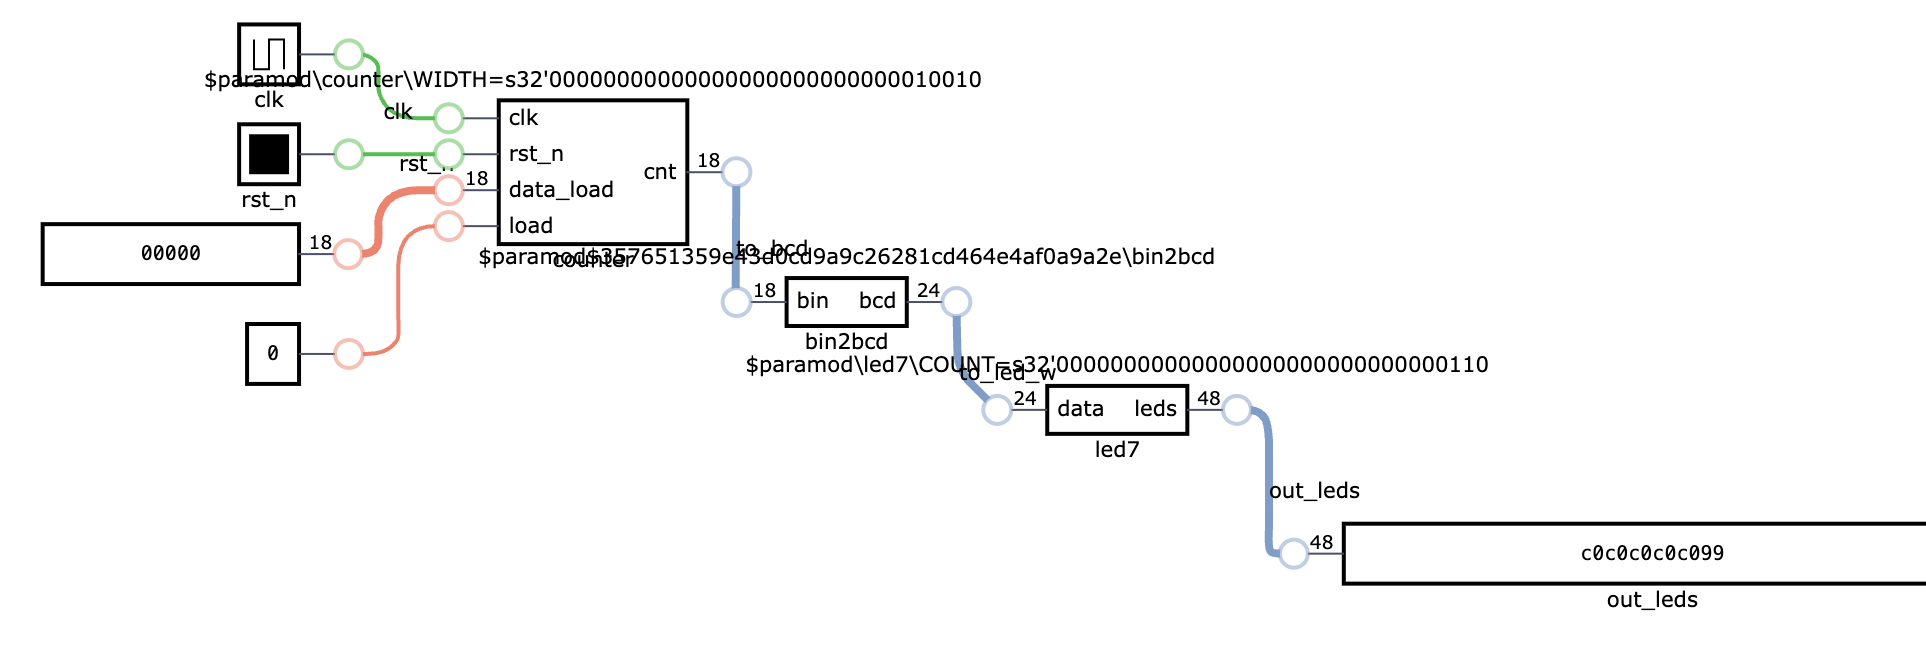
\includegraphics[width=0.9\textwidth]{lab_323.png}
    \caption{RTL}
  \end{figure}

  \begin{listing}[H]
    \begin{minted}{cpp}
      // ====================  Testbench   ====================

      task->rst_n = 1; nextStep();

      for (int i = 0; i < 1325; i++) {
          printLedsWire(task->out_leds);
          nextPeriod();
      }

      task->rst_n = 0; nextStep();
      printLedsWire(task->out_leds);
    \end{minted}
    \caption{Код тестбенча}
  \end{listing}

  \begin{listing}[H]
    \begin{minted}{verilog}
       _  _  _  _  _  _ 
      | || || || || || |
      | || || || || || |
       ‾  ‾  ‾  ‾  ‾  ‾ 
       _  _  _  _  _    
      | || || || || |  |
      | || || || || |  |
       ‾  ‾  ‾  ‾  ‾    
      ...
          _  _  _  _  _ 
        || || || | _||_|
        || || || ||    |
          ‾  ‾  ‾  ‾  ‾ 
       _  _  _  _  _  _ 
      | || || || || || |
      | || || || || || |
       ‾  ‾  ‾  ‾  ‾  ‾ 
    \end{minted}
    \caption{Результат работы тестбенча}
  \end{listing}

  \begin{figure}[H]
    \centering
    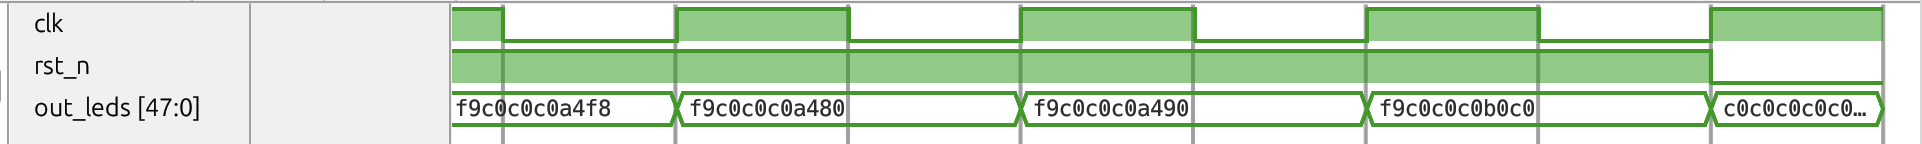
\includegraphics[width=0.9\textwidth]{lab_324}
    \caption{Результат работы тестбенча}
  \end{figure}

  \subsection{Отображение на всех разрядах группы семисегментных индикаторов одного и того же значения со счётчика (задание 3)}

  \begin{listing}[H]
    \inputminted{verilog}{../chapter_6/extra/3/task3.v}
    \caption{Счётчик, значение которого выводится на несколько семисегментных индикаторов}
  \end{listing}

  \begin{figure}[H]
    \centering
    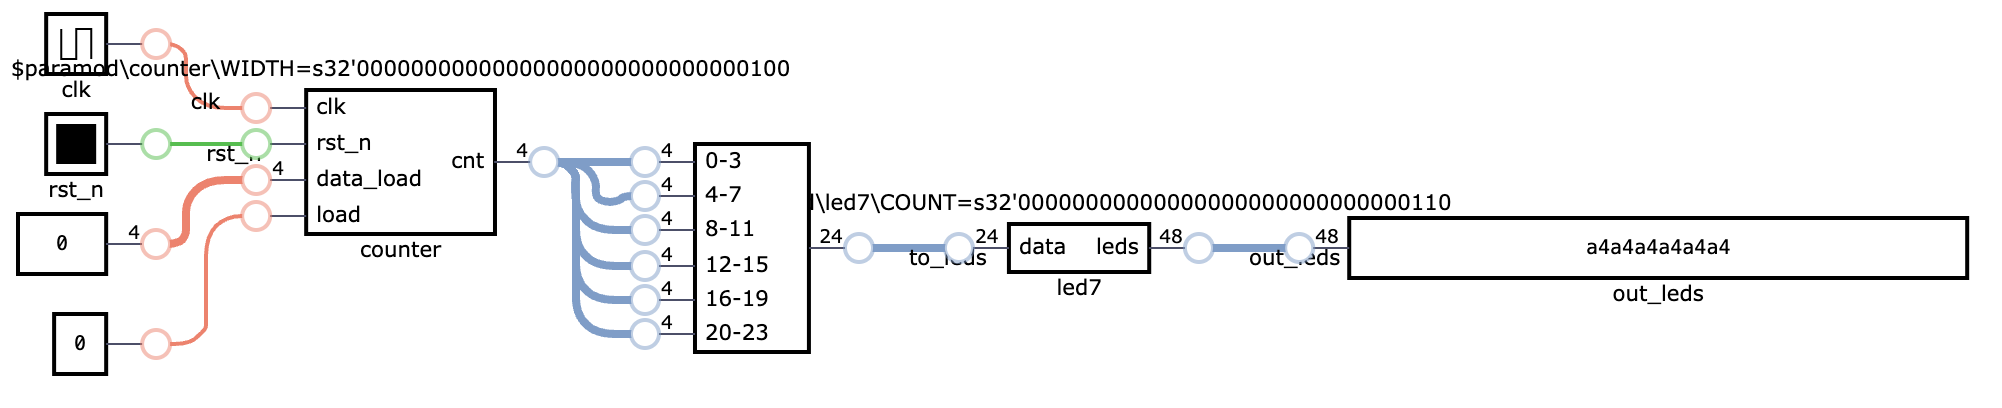
\includegraphics[width=0.9\textwidth]{lab_325.png}
    \caption{RTL}
  \end{figure}

  Код тестбенча аналогичен предыдущему заданию.

  \begin{listing}[H]
    \begin{minted}{text}
     _  _  _  _  _  _ 
    | || || || || || |
    | || || || || || |
     ‾  ‾  ‾  ‾  ‾  ‾ 
                      
      |  |  |  |  |  |
      |  |  |  |  |  |
    ...
     _  _  _  _  _  _ 
    |_ |_ |_ |_ |_ |_ 
    |  |  |  |  |  |  
               
     _  _  _  _  _  _ 
    | || || || || || |
    | || || || || || |
     ‾  ‾  ‾  ‾  ‾  ‾ 
    \end{minted}
    \caption{Результат работы тестбенча}
  \end{listing}

  \begin{figure}[H]
    \centering
    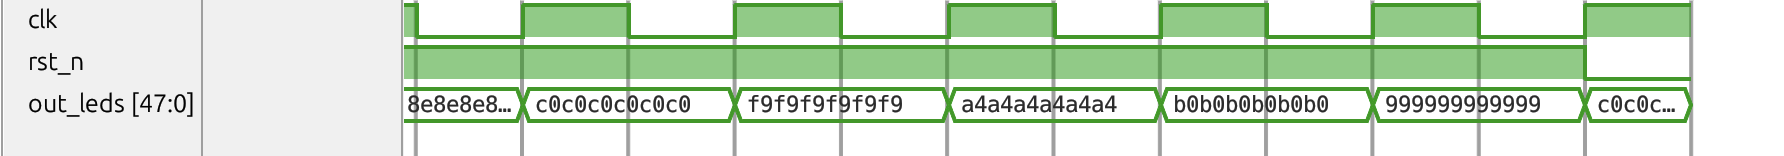
\includegraphics[width=0.9\textwidth]{lab_326}
    \caption{Результат работы тестбенча}
  \end{figure}

  \subsection{Подключение счётчика Грея к группе нескольких семисегментных индикаторов (задание 10)}

  Код Грея - код, состоящий только из нулей и единиц, поэтому не получится просто соединить
  счётчик и дешифратор, чтобы вывести необходимые значения. Необходимо
  разбить код с выхода на несколько отдельных символов:

  \begin{listing}[H]
    \inputminted{verilog}{../chapter_6/extra/10/task10.v}
    \caption{Реализация решения}
  \end{listing}

  \begin{figure}[H]
    \centering
    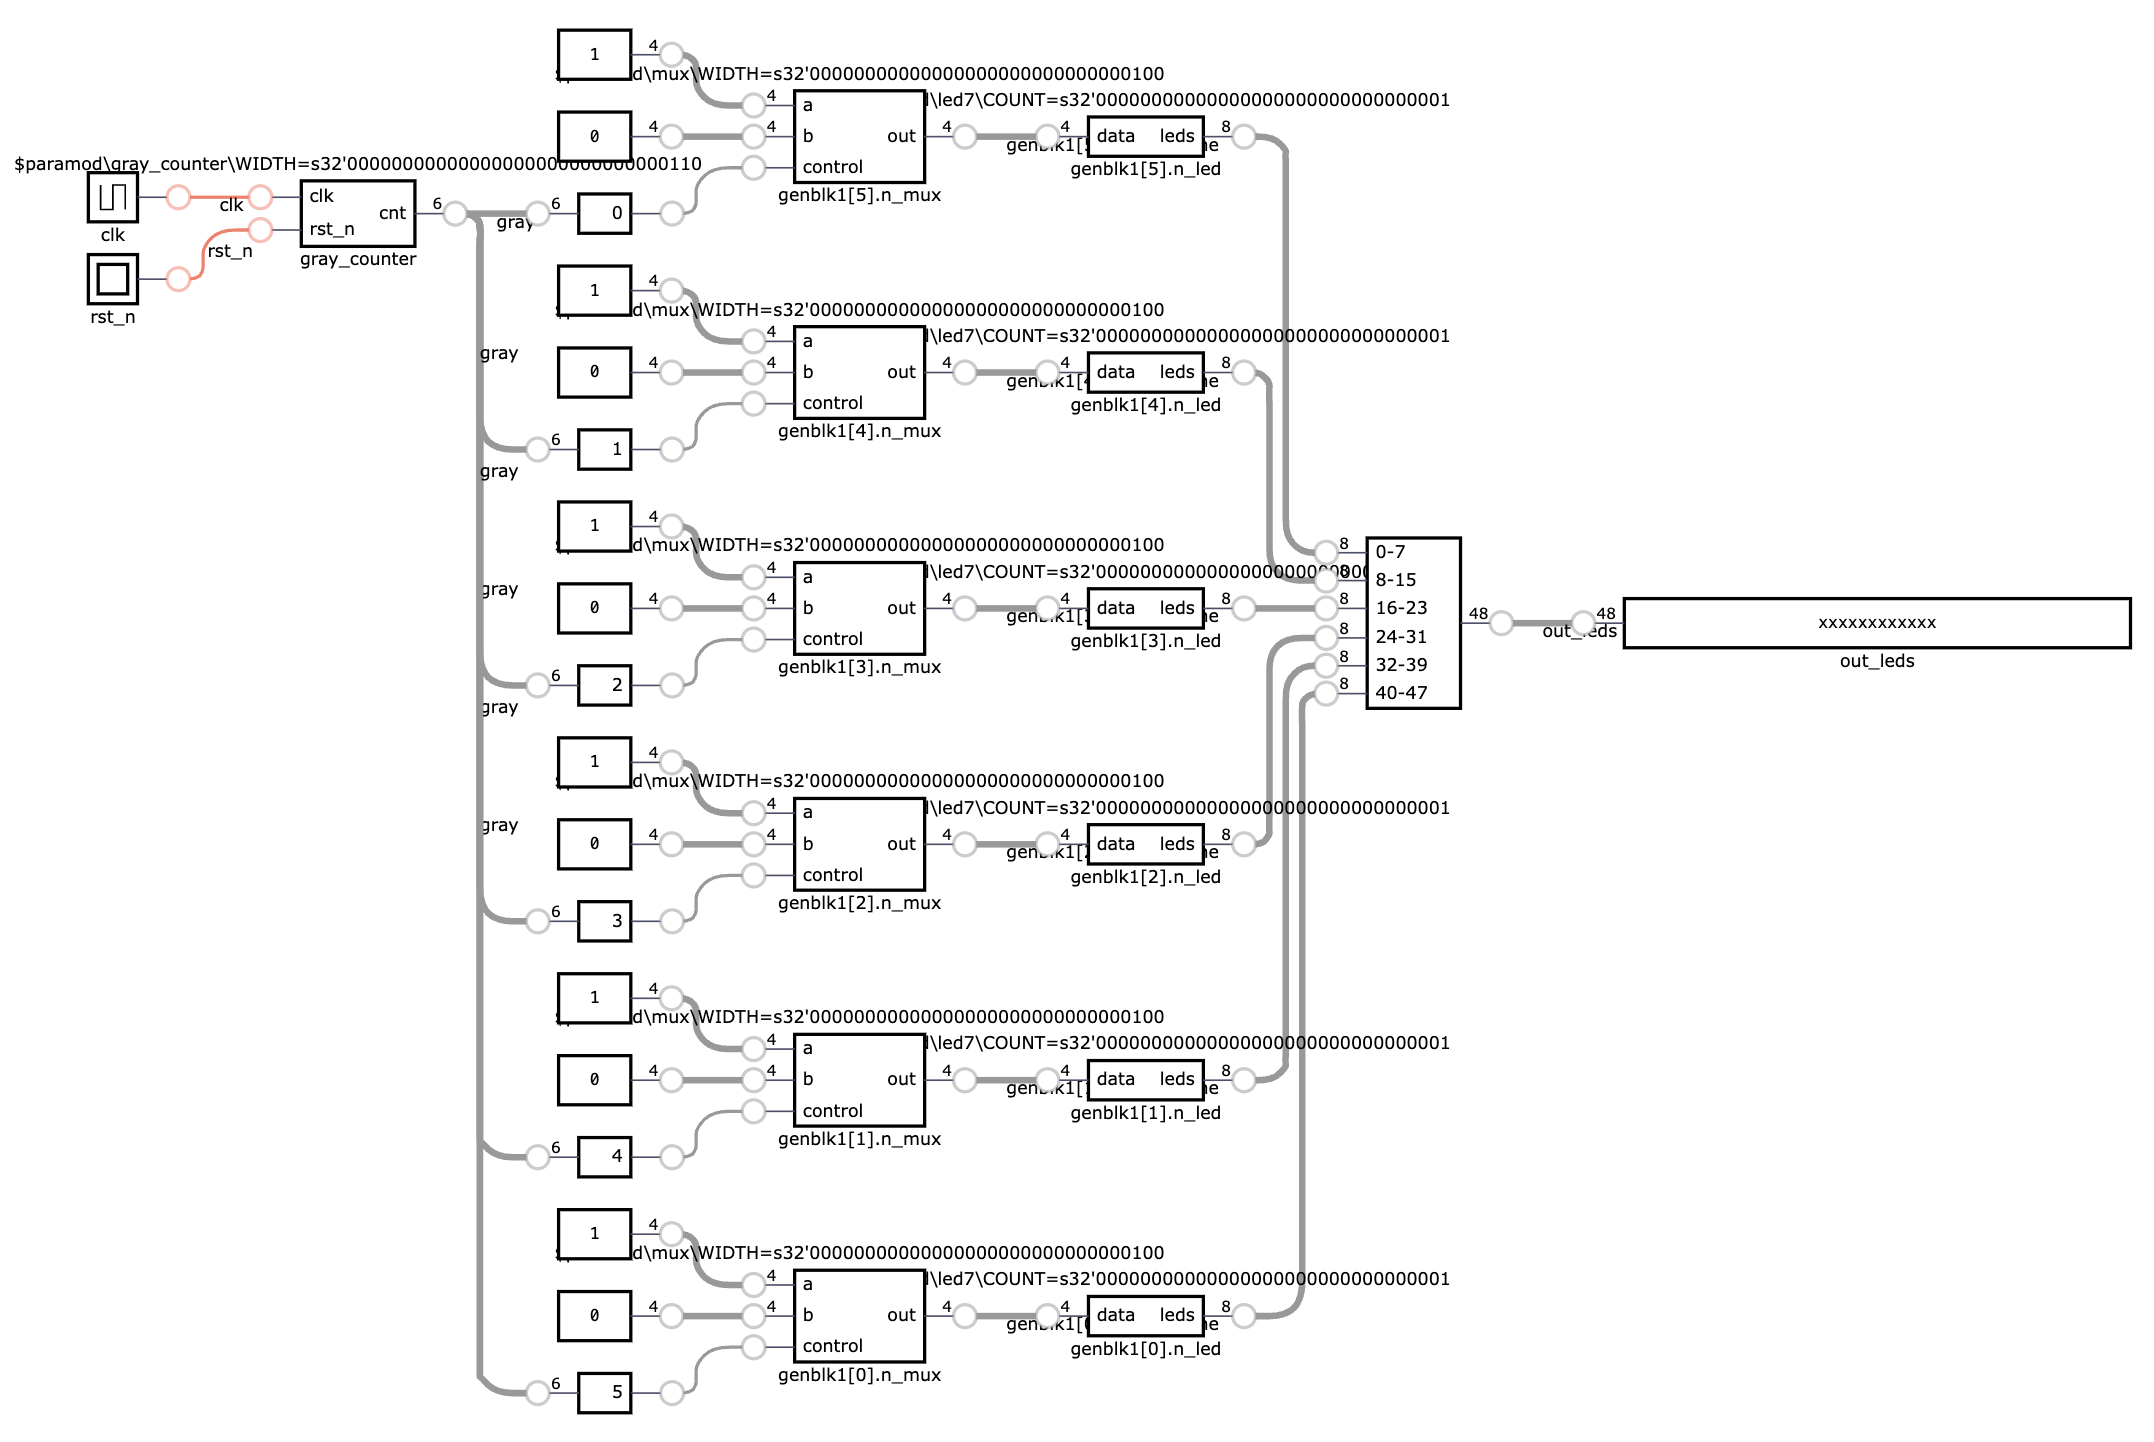
\includegraphics[width=0.9\textwidth]{lab_327.png}
    \caption{RTL}
  \end{figure}

  Код тестбенча аналогичен предыдущим двум примерам.

  \begin{listing}[H]
    \begin{minted}{text}
       _  _  _  _  _  _ 
      | || || || || || |
      | || || || || || |
       ‾  ‾  ‾  ‾  ‾  ‾ 
       _  _  _  _  _    
      | || || || || |  |
      | || || || || |  |
       ‾  ‾  ‾  ‾  ‾    
       _  _  _  _       
      | || || || |  |  |
      | || || || |  |  |
       ‾  ‾  ‾  ‾       
       _  _  _  _     _ 
      | || || || |  || |
      | || || || |  || |
       ‾  ‾  ‾  ‾     ‾ 
      ...
    \end{minted}
    \caption{Результат работы тестбенча}
  \end{listing}

  \begin{figure}[H]
    \centering
    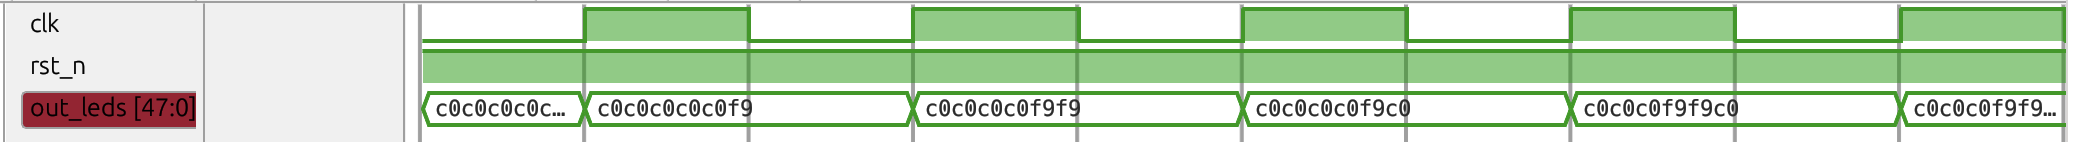
\includegraphics[width=0.9\textwidth]{lab_328}
    \caption{Результат работы тестбенча}
  \end{figure}

  \subsection{Сдвиговый регистр с управляемым по нажатию кнопки направлением сдвига (задание 13)}

  Для того, чтобы детектировать краткосрочные нажатия на кнопку, воспользуется T-триггером:
  \begin{listing}[H]
    \inputminted{verilog}{../chapter_6/extra/13/t_flip_flop.v}
    \caption{T-триггер}
  \end{listing}

  Также необходимо улучшить сдвиговый регистр, чтобы он сомг изменять направление сдвига:
  \begin{listing}[H]
    \inputminted{verilog}{../chapter_6/extra/13/shift_directional_register.v}
    \caption{Сдвиговый регистр с поддержкой изменения направления сдвига}
  \end{listing}

  \begin{listing}[H]
    \inputminted{verilog}{../chapter_6/extra/13/task13.v}
    \caption{Реализация задания}
  \end{listing}

  \begin{figure}[H]
    \centering
    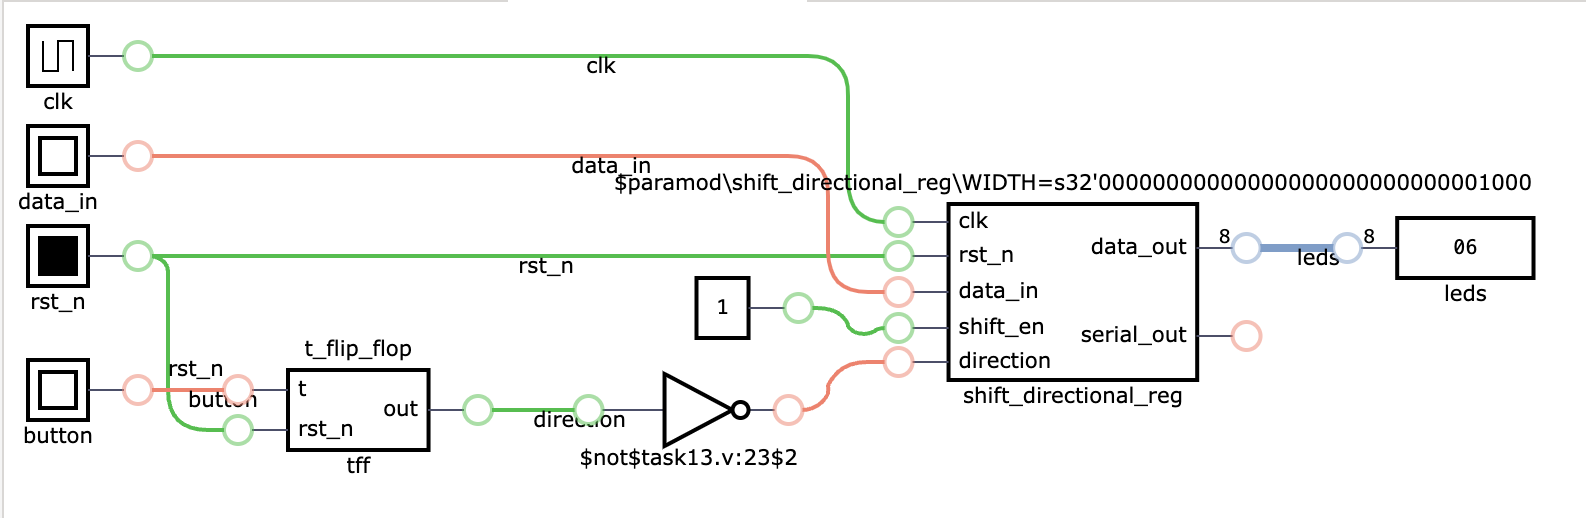
\includegraphics[width=0.9\textwidth]{lab_329.png}
    \caption{RTL}
  \end{figure}

  \begin{listing}[H]
    \begin{minted}{cpp}
// ====================  Testbench   ====================

task->rst_n = task->data_in = 1;

for (int i = 0; i < 16; i++) {
    showLeds(task->leds);
    nextPeriod();
    if (i % 5 == 4) {
        task->data_in = task->data_in ? 0 : 1;
    }
    if (i == 10) {
        std::cout << "Clk" << std::endl;
        task->button = 1;
    } else if (i == 11) {
        task->button = 0;
    }
}
    \end{minted}
    \caption{Основная часть тестбенча}
  \end{listing}

  \begin{listing}[H]
    \begin{minted}{text}
      --------
      #-------
      ##------
      ###-----
      ####----
      #####---
      -#####--
      --#####-
      ---#####
      ----####
      -----###
      Clk
      #-----##
      -----###
      ----####
      ---#####
      --######
    \end{minted}
    \caption{Результат работы тестбенча}
  \end{listing}

  \begin{figure}[H]
    \centering
    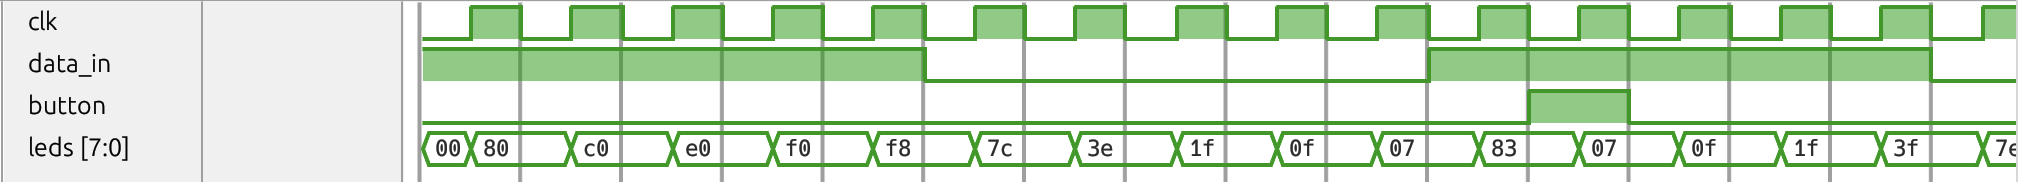
\includegraphics[width=0.9\textwidth]{lab_330.png}
    \caption{Результат работы тестбенча}
  \end{figure}

  \newpage
  \section{Выводы}

  В результате данной работы были реализованы различные виды счётчиков, на их основе был выполнен ШИМ и делитель частоты.

\end{document}
